\documentclass[11pt]{article}
\usepackage[T1]{fontenc}
\usepackage[utf8]{inputenc}
\usepackage[spanish,es-tabla]{babel}
\usepackage[margin=2.5cm]{geometry}
\usepackage{graphicx}
\usepackage{array}

\title{Servicio de paquetería\\ \large Documento de diseño, Tema 3}
\author{Martínez Aguilar Carlos Alain \\ Gonzalez Morales Daniel Alejandro \\
Garces Diaz Gustavo Osei \\ Garcia Bizueto Sebastian}
\date{}

\begin{document}
\maketitle

\section{Diagramas UML}

\subsection{Diagrama de clases}
\noindent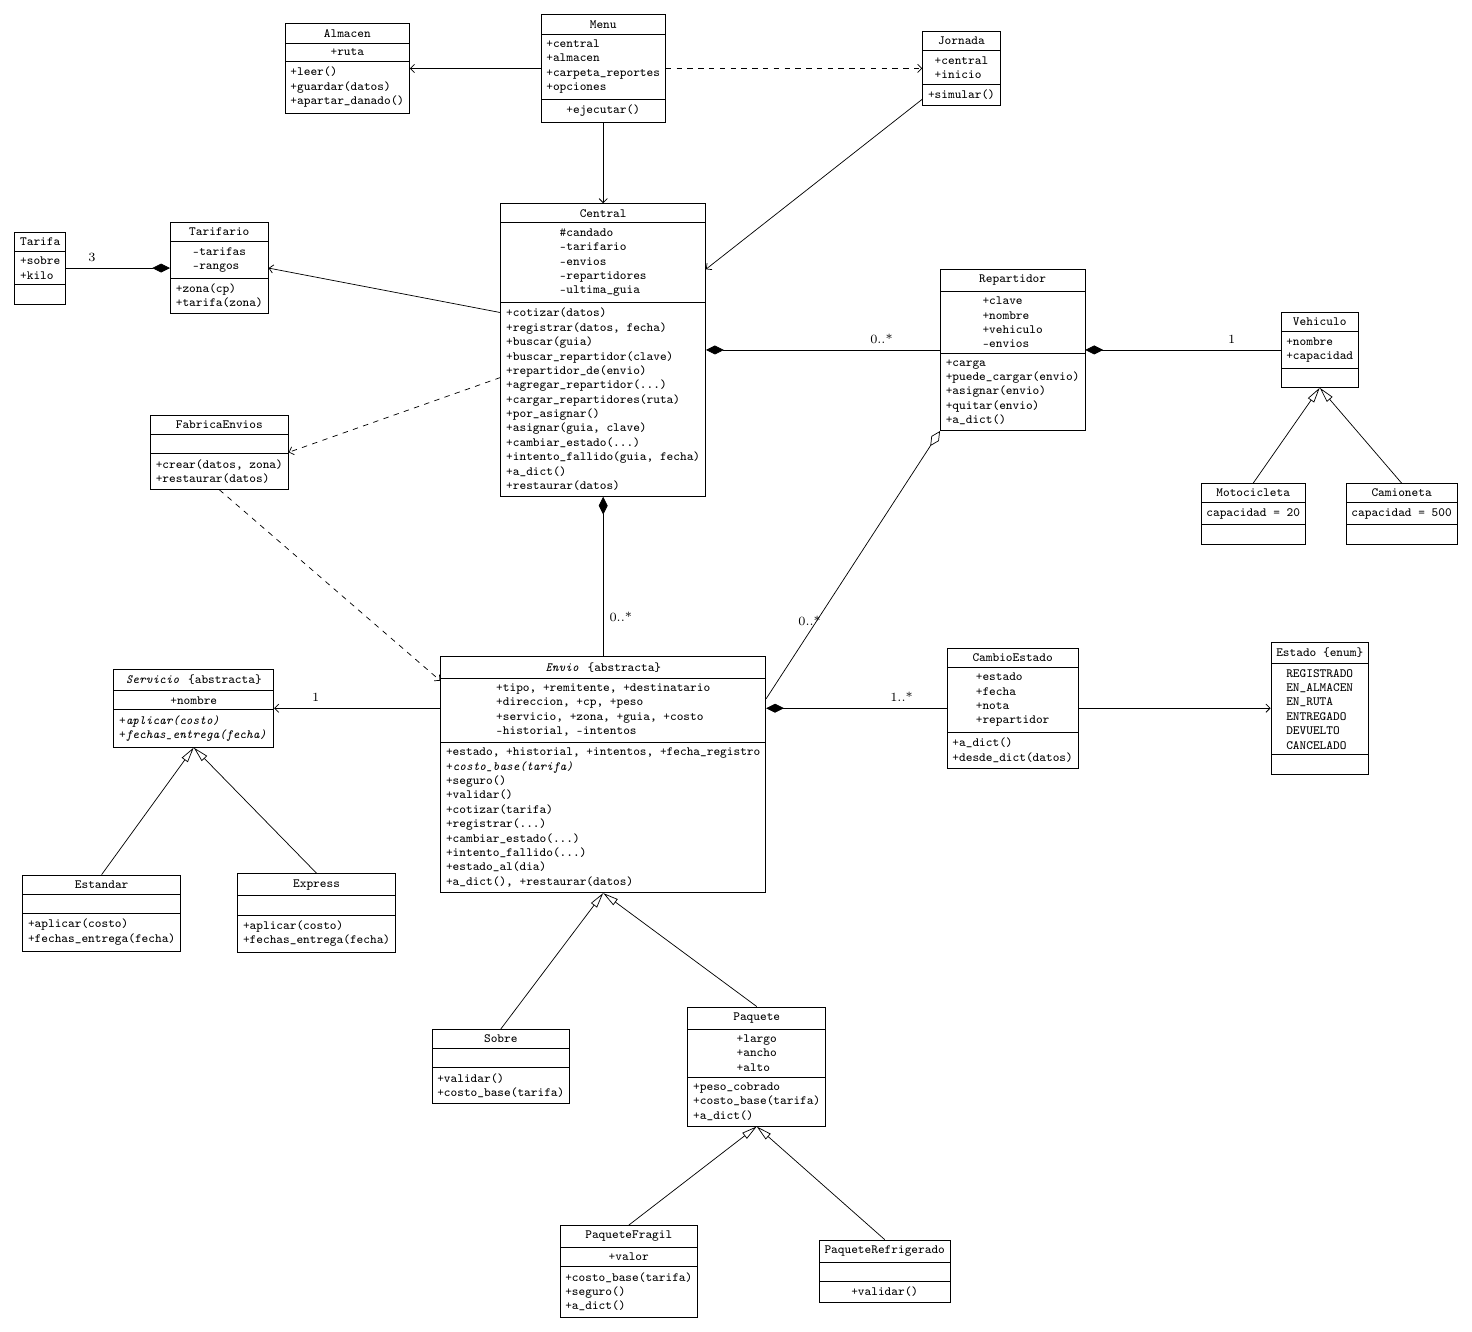
\includegraphics[width=\textwidth]{uml/clases.png}

Muestra las clases, sus atributos, sus métodos y cómo se relacionan. Se eligió porque es donde se ve qué hace
cada parte del sistema.

\subsection{Diagrama de estados}
\noindent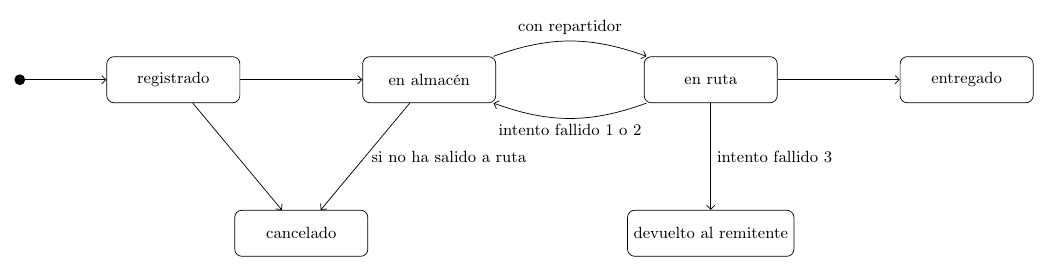
\includegraphics[width=\textwidth]{uml/estados.png}

Muestra por qué estados pasa un envío. Se eligió porque la mayoría de los rechazos dependen del estado.

\subsection{Diagrama de secuencia}
Por completar (Sebastian): jornada de reparto.

\section{Decisiones de diseño}

\begin{center}
\small
\renewcommand{\arraystretch}{1.3}
\begin{tabular}{|>{\raggedright\arraybackslash}p{3cm}|>{\raggedright\arraybackslash}p{5cm}|>{\raggedright\arraybackslash}p{5.3cm}|}
\hline
\textbf{Concepto} & \textbf{Dónde se usa} & \textbf{Qué problema resuelve} \\ \hline
Encapsulamiento & Historial e intentos de \texttt{Envio}, envíos de \texttt{Repartidor} & El estado y la carga solo cambian con métodos que revisan las reglas \\ \hline
Herencia y clases abstractas & \texttt{Envio} y sus tipos, \texttt{Servicio}, \texttt{Vehiculo} & Cada tipo solo define lo que lo hace distinto \\ \hline
Composición y agregación & \texttt{Envio} tiene su historial; \texttt{Repartidor} agrupa envíos & El historial no existe sin el envío; el envío sí existe sin repartidor \\ \hline
Polimorfismo & \texttt{costo\_base}, \texttt{seguro}, \texttt{validar}, \texttt{aplicar} & La central cotiza sin preguntar el tipo de envío \\ \hline
Excepciones & \texttt{excepciones.py} & El menú atrapa un solo error base y muestra el motivo \\ \hline
Archivos & \texttt{leer\_csv}, \texttt{Almacen} & Cargar tarifas y conservar los datos; se escribe en un temporal para no dañar lo guardado \\ \hline
Hilos & Candado de \texttt{Central}; jornada por completar (Sebastian) & Dos repartidores no modifican los datos al mismo tiempo \\ \hline
Patrones de diseño & \texttt{FabricaEnvios} (Factory), \texttt{Servicio} (Strategy), \texttt{cotizar} (Template Method), \texttt{Central} (Facade) & Crear el tipo correcto, cambiar el precio según el servicio y que el menú use una sola clase \\ \hline
\end{tabular}
\end{center}

\subsection{Detalles que decidimos}
\begin{itemize}
\item El 50\,\% de express se aplica al costo y al 20\,\% de frágil, pero no al seguro.
\item Los días de entrega son naturales.
\item Un sobre pesa máximo 1 kg y un paquete 500 kg, que es lo que carga una camioneta.
\item La capacidad se revisa con el peso real.
\item La zona es la del primer rango de \texttt{zonas.csv} que contiene el código postal. El origen es la Ciudad de México.
\item Un envío necesita repartidor para salir a ruta. Si la entrega falla, se queda sin repartidor.
\item Un envío que ya salió a ruta no se cancela aunque haya regresado al almacén.
\item Un cambio no puede tener una fecha anterior al último cambio del envío.
\end{itemize}

\section{Alternativas}
\begin{itemize}
\item \textbf{Estados con un diccionario o con una clase por estado.} Se eligió el diccionario porque los estados
casi no tienen comportamiento propio y así las reglas se leen en un solo lugar.
\item \textbf{JSON o CSV para guardar.} Se eligió JSON porque el historial es una lista dentro de cada envío y en
CSV harían falta varios archivos relacionados.
\end{itemize}

\section{Uso de IA}
\begin{itemize}
\item Qué se pidió: a partir del enunciado, el código base, los datos de ejemplo, los diagramas y esta documentación.
\item Qué se usó: la primera versión de los módulos de \texttt{modelos}, \texttt{archivos}, \texttt{central},
\texttt{tarifario}, \texttt{fabrica}, \texttt{menu} y \texttt{main}.
\item Qué se corrigió: por completar por el equipo.
\item Cómo se verificó: se ejecutaron los casos del README, incluidos los rechazos y los archivos dañados.
\end{itemize}

\section{Contribuciones}
\begin{itemize}
\item Martínez Aguilar Carlos Alain: por completar.
\item Gonzalez Morales Daniel Alejandro: por completar.
\item Garces Diaz Gustavo Osei: por completar.
\item Garcia Bizueto Sebastian: por completar.
\end{itemize}

\end{document}
